In this section the governing model equations for the x and y axes is Laplace transformed and put on transfer function. 
\subsection*{Roll translational controller}
For the sake of repetition, the model expression for the roll is as follows:
\begin{align}
m\cdot\Delta\ddot{x}_I = -k_{th}\cdot({\overline{\omega}_1}^2+{\overline{\omega}_2}^2+{\overline{\omega}_3}^2+{\overline{\omega}_4}^2)\cdot\cos(\overline{\theta})\Delta\theta
\label{eq:model_x_transl}
\end{align} 
Laplace transforming \autoref{eq:model_x_transl} yields:
\begin{align}
m\cdot x_1(s)s^2=-k_{th}\cdot (\omega_1 ^2 + \omega_2 ^2 + \omega_3 ^2 + \omega_4 ^2)\cdot \theta
\end{align}
It is desirable to have a transfer function where the input is the roll angle as this is the output from the attitude controller that goes into the translational controller block. The output of the translational pitch controller must be the velocity in the x axes. \\
The transfer function can now be written as:
\begin{align}
H_{x1}(s)=\frac{x_1(s) \cdot s}{\theta}=\frac{k_{th}\cdot (\omega_1 ^2 + \omega_2 ^2 + \omega_3 ^2 + \omega_4 ^2)}{m\cdot s}\label{eq:conHx}
\end{align}
\begin{where}
\va{H_{x1}}{is the plant for the translational roll}{1}
\end{where}
 
Limit check of the transfer function to verify if the model behaves as the plant is expected to in reality. \\\\
\fxfatal{I am having trouble thinking about it, as it is not entirely intuitive to me, when the input is an angle and not a force - however if possible, i think we should have a short piece of text to show we have been critical to the math we have derived - to check it before continuing.} 


As it can be seen from \autoref{eq:conHx}, the submodel of the translational roll has a pole in zero. This makes it a type 1 system, which means no steady state error will be present in its step response. 
A proportional controller is considered sufficient, as it does not have to compensate for a steady state error. By increasing the gain the system will become faster, which is desirable. To determine how large the gain can be without making the system unstable by saturation issues, it is necessary to consider the bandwidth. \newpar
The data from the Vicon is transmitted with 100 Hz. This means the attitude controller must run with 50 Hz as maximum to ensure the controller is slower than the sensor data. A rule of thumb states that the bandwidth of the system shall be 25 times smaller than the attitude controller. The desired bandwidth of the translational roll controller is calculated as follows:
\begin{align}
BW=2\cdot \pi\cdot \frac{f_s}{25}=2\cdot \pi \frac{50}{25}=12.57\label{eq:bw_X}
\end{align}
\begin{where}
\va{BW}{is the bandwidth of the plant}{rad \cdot s^{-1}}
\va{f_s}{is the sampling frequency of the plant}{Hz}
\end{where}

From \autoref{eq:bw_X} it is known, that the ideal bandwidth of the system is 12.57 rad/s. 
\begin{figure}[H]
	\centering
	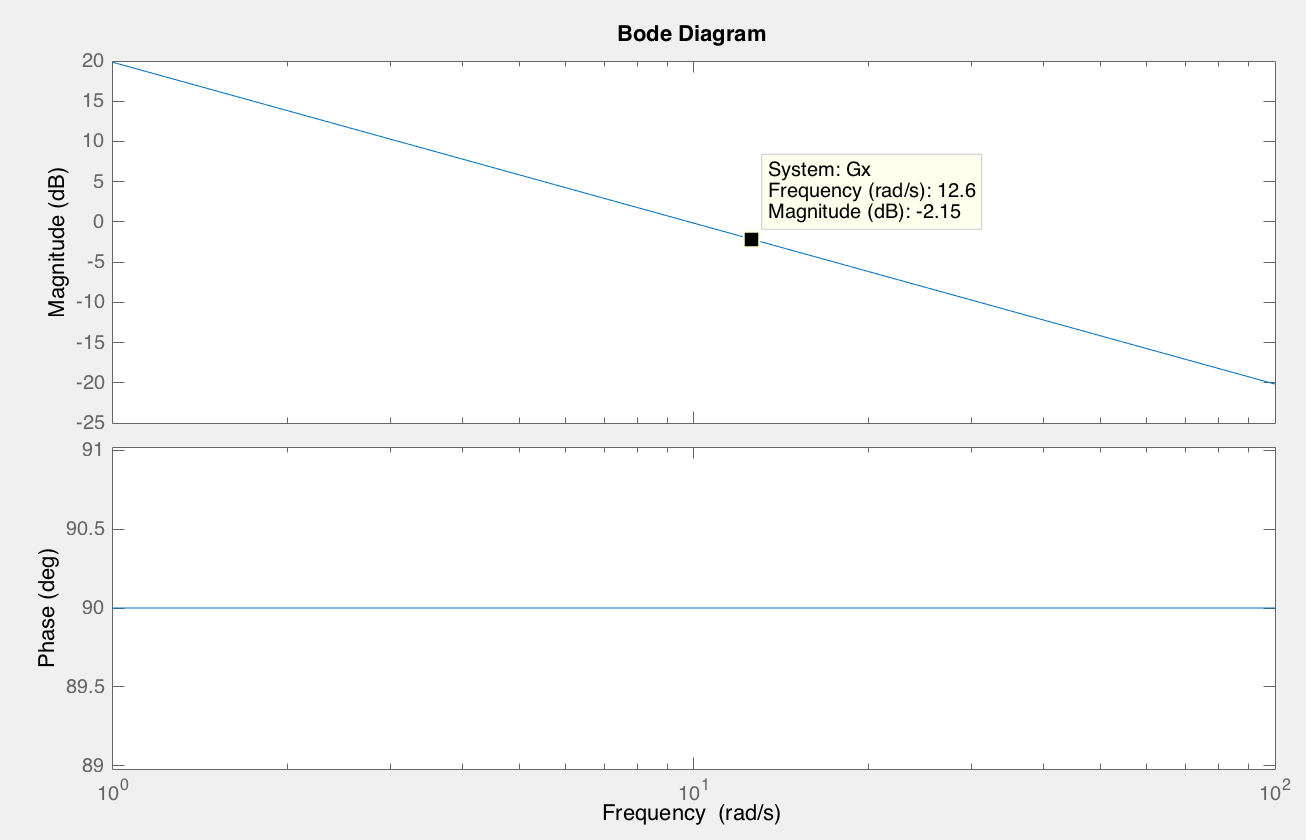
\includegraphics[width=0.8\textwidth]{figures/bode_x.png}
	\caption{Bodeplot of the plant, with the bandwidth of 12.6 rad/s displayed.}\label{fig:bode_x}
\end{figure}
The bodeplot in \autoref{fig:bode_x} reveals that the magnitude is 2.15 dB at 12.6 rad/s and must be lifted by 

\subsection*{Pitch translational controller}
The model expression for pitch is previously derived to be:
\begin{align}
m\cdot\Delta\ddot{y}_I = k_{th}\cdot({\overline{\omega}_1}^2+{\overline{\omega}_2}^2+{\overline{\omega}_3}^2+{\overline{\omega}_4}^2)\cdot\cos(\overline{\phi})\cdot\cos(\overline{\theta})\cdot\Delta\phi
\label{eq:model_y_transl}
\end{align}
Laplace transforming \autoref{eq:model_y_transl_y} yields:
\begin{align}
m\cdot y_1(s)\cdot s^2= k_{th}\cdot (\omega_1 ^2 + \omega_2 ^2 + \omega_3 ^2 + \omega_4 ^2)\cdot \phi
\end{align}
The transfer function for the pitch is as follows:
\begin{align}
H_{y1}(s)=\frac{y_1(s)\cdot s}{\phi}=\frac{k_{th}\cdot (\omega_1 ^2 + \omega_2 ^2 + \omega_3 ^2 + \omega_4 ^2)}{m\cdot s}
\end{align}
\begin{where}
\va{H_{y1}}{is the plant for the translational pitch}{1}
\end{where}
 
Root locus and bode and all that and we end up with P controller

simulation of the controllers